
\documentclass[xcolor=dvipsnames]{beamer} % dvipsnames gives more built-in colors
\usepackage[utf8]{inputenc}
\usepackage[spanish]{babel}

\mode<presentation> {

\usetheme{CambridgeUS}

%\setbeamertemplate{footline} % To remove the footer line in all slides uncomment this line
\setbeamertemplate{footline}[page number] % To replace the footer line in all slides with a simple slide count uncomment this line

\setbeamertemplate{navigation symbols}{} % To remove the navigation symbols from

\definecolor{utfsmred}{HTML}{D60019}
\definecolor{utfsmyellow}{HTML}{F7AE00}
\definecolor{utfsmgreen}{HTML}{008452}
\definecolor{utfsmblue}{HTML}{004B85}


\newenvironment<>{rosa}[1][]{
  \setbeamercolor{block title example}{fg=white,bg=blue!75!black}%
  \begin{example}#2[#1]}{
  \end{example}
}

\usepackage{hyperref}
\definecolor{links}{HTML}{2A1B81}
\hypersetup{colorlinks,linkcolor=,urlcolor=links}

\usecolortheme[named=utfsmblue]{structure}
\setbeamercolor{titlelike}{parent=structure,fg=utfsmblue}
\setbeamercolor{frametitle}{fg=utfsmblue}

%\setbeamercolor{section in head/foot}{bg=Brown}
%\setbeamercolor{author in head/foot}{bg=Brown}
%\setbeamercolor{date in head/foot}{fg=Brown}

\setbeamercolor*{enumerate item}{fg=utfsmred}
\setbeamercolor*{enumerate subitem}{fg=utfsmred}
\setbeamercolor*{enumerate subsubitem}{fg=utfsmred}

\setbeamercolor*{itemize item}{fg=utfsmred}
\setbeamercolor*{itemize subitem}{fg=utfsmred}
\setbeamercolor*{itemize subsubitem}{fg=utfsmred}

\setbeamercolor{item projected}{bg=utfsmred}


\setbeamertemplate{itemize items}[square]
\setbeamertemplate{enumerate items}[default]


\setbeamercolor{section in head/foot}{bg=utfsmblue}

\setbeamercolor{block title}{bg=utfsmblue!80,fg=white}
\setbeamercolor{block title alerted}{bg=utfsmred!80,fg=white}
\setbeamercolor{block title example}{bg=utfsmgreen!80,fg=white}

\setbeamertemplate{sections/subsections in toc}[square]
\setbeamercolor{section number projected}{bg=utfsmblue,fg=white}


}

\usepackage[normalem]{ulem}

\usepackage{graphicx} % Allows including images
\usepackage{booktabs} % Allows the use of \toprule, \midrule and \bottomrule in tables
\usepackage{listings}
\lstset{ %
language=C,
basicstyle=\normalsize\ttfamily,
keywordstyle=,
numbers=none,
numberstyle=\tiny\ttfamily,
stepnumber=1,
showspaces=false,
showstringspaces=false,
showtabs=false,
breaklines=true,
frame=tb,
framerule=0.5pt,
tabsize=4,
framexleftmargin=0.5em,
framexrightmargin=0.5em,
xleftmargin=0.5em,
xrightmargin=0.5em,
}

%----------------------------------------------------------------------------------------
%	TITLE PAGE
%----------------------------------------------------------------------------------------

\title{MySQL Performance Tuning}
\subtitle{\small{Seminario de Desarrollo de Software - Casa Central.}}
\author{Maximiliano Osorio\\\small{mosorio@inf.utfsm.cl}} 
\institute[UTFSM]
{
Universidad Técnica Federico Santa María
\medskip
}
\date{\today} % Date, can be changed to a custom date

\begin{document}
	
%-=-=-=-=-=-=-=-=-=-=-=-=-=-=-=-=-=-=-=-=-=-=-=-=
%
%	TITLE PAGE
%
%-=-=-=-=-=-=-=-=-=-=-=-=-=-=-=-=-=-=-=-=-=-=-=-=





%\begin{block}{Dependencias}
%\end{block}
\maketitle
\section{Dummy mistakes}

\begin{frame}[fragile]
\frametitle{Mistakes}

\begin{block}{Change one setting at a time!}
This is the only way to estimate if a change is beneficial.
\end{block}

\end{frame}
%------------------------------------------------

\begin{frame}[fragile]
\frametitle{Mistakes}

\begin{block}{SET GLOBAL.}
Most settings can be changed at runtime with SET GLOBAL. It is very handy and it allows you to quickly revert the change if it creates any problem
\end{block}

\begin{alertblock}{Caution}
But in the end, you want the setting to be adjusted permanently in the configuration file.
\end{alertblock}


\end{frame}

%------------------------------------------------

\begin{frame}[fragile]
\frametitle{Mistakes}

\begin{block}{A change in the configuration is not visible even after a MySQL restart}
 Did you use the correct configuration file? Did you put the setting in the right section? (all settings in this post belong to the [mysqld] section)
\end{block}

\end{frame}

%------------------------------------------------

\begin{frame}[fragile]
\frametitle{Mistakes}

\begin{block}{Do not allow duplicate settings in the configuration file.}
If you want to keep track of the changes, use version control.
\end{block}

\end{frame}

%------------------------------------------------

\section{Basic settings}
\subsection{innodb\_buffer\_pool\_size}
\begin{frame}[fragile]
\frametitle{innodb\_buffer\_pool\_size:}

\begin{itemize}
  \item this is the \#1 setting to look at for any installation using InnoDB.
\end{itemize}

\begin{block}{Definition}
 The buffer pool is where data and indexes are cached: having it as large as possible will ensure you use memory and not disks for most read operations.
\end{block}

\end{frame}

%------------------------------------------------

\begin{frame}[fragile]
\frametitle{Typical values}
Typical values are:
\begin{itemize}
  \item 5-6GB (8GB RAM)
  \item 20-25GB (32GB RAM)
  \item 100-120GB (128GB RAM)
\end{itemize}

\end{frame}

%------------------------------------------------

\subsection{innodb\_log\_file\_size}

\begin{frame}[fragile]
\frametitle{innodb\_log\_file\_size}

\begin{block}{Definition}
This is the size of the redo logs. The redo logs are used to make sure writes are fast and durable and also during crash recovery.
\end{block}


\end{frame}
%------------------------------------------------

\begin{frame}[fragile]
\frametitle{Typical values}
\begin{itemize}
  \item Starting with innodb\_log\_file\_size = 512M (giving 1GB of redo logs) should give you plenty of room for writes. 
  \item If you know your application is write-intensive and you are using MySQL 5.6, you can start with innodb\_log\_file\_size = 4G.
\end{itemize}

\end{frame}
%------------------------------------------------

\subsection{max\_connections}

\begin{frame}[fragile]
\frametitle{max\_connections}

\begin{itemize}
  \item  if you are often facing the Too many connections error, max\_connections is too low.
  \item  It is very frequent that because the application does not close connections to the database correctly, you need much more than the default 151 connections. 
  \item The main drawback of high values for max\_connections (like 1000 or more) is that the server will become unresponsive if for any reason it has to run 1000 or more active transactions.
\end{itemize}

\end{frame}
%------------------------------------------------

\section{InnoDB settings}

\begin{frame}[fragile]
\frametitle{InnoDB}
InnoDB has been the default storage engine since MySQL 5.5 and it is much more frequently used than any other storage engine. That’s why it should be configured carefully.

\end{frame}
%------------------------------------------------


\begin{frame}[fragile]
\frametitle{innodb\_file\_per\_table}

\begin{block}{Definition}
This setting will tell InnoDB if it should store data and indexes in the shared tablespace (innodb\_file\_per\_table = OFF) or in a separate .ibd file for each table (innodb\_file\_per\_table= ON)
\end{block}

\end{frame}
%------------------------------------------------


\begin{frame}[fragile]
\frametitle{innodb\_file\_per\_table}

\begin{itemize}
  \item Having a file per table allows you to reclaim space when dropping, truncating or rebuilding a table. It is also needed for some advanced features such as compression. However it does not provide any performance benefit
  \item The main scenario when you do NOT want file per table is when you have a very high number of tables (say 10k+).

\end{itemize}

\end{frame}
%------------------------------------------------

\begin{frame}[fragile]
\frametitle{innodb\_flush\_log\_at\_trx\_commit}

\begin{itemize}
  \item the default setting of 1 means that InnoDB is fully ACID compliant. It is the best value when your primary concern is data safety
  \item However it can have a significant overhead on systems with slow disks because of the extra fsyncs
  \item Setting it to 2 is a bit less reliable because committed transactions will be flushed to the redo logs only once a second
  \item 0 is even faster but you are more likely to lose some data in case of a crash: it is only a good value for a replica.
\end{itemize}


\end{frame}
%------------------------------------------------


\begin{frame}[fragile]
\frametitle{innodb\_flush\_method}
This setting controls how data and logs are flushed to disk,  popular values are 
\begin{itemize}
  \item O\_DIRECT when you have a hardware RAID controller with a battery-protected write-back cache
  \item  fdatasync (default value) for most other scenarios. 
\end{itemize}
sysbench is a good tool to help you choose between the 2 values
\end{frame}
%------------------------------------------------


\begin{frame}[fragile]
\frametitle{}
\begin{figure}
\centering
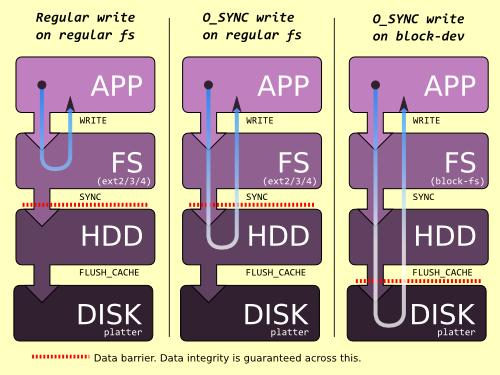
\includegraphics[width=\textwidth,height=1\textheight,keepaspectratio]{images/data-barriers-hdd-write
}
\end{figure}

\end{frame}
%------------------------------------------------


\begin{frame}[fragile]
\frametitle{innodb\_log\_buffer\_size}
this is the size of the buffer for transactions that have not been committed yet. 
\begin{itemize}
  \item The default value (1MB) is usually fine but as soon as you have transactions with large blob/text fields, the buffer can fill up very quickly and trigger extra I/O load
\end{itemize}
Look at the Innodb\_log\_waits status variable and if it is not 0, increase innodb\_log\_buffer\_size.

\end{frame}
%------------------------------------------------


\section{Other settings}
\subsection{query\_cache\_size}
\begin{frame}[fragile]
\frametitle{query\_cache\_size}

the query cache is a well known bottleneck that can be seen even when concurrency is moderate

\begin{itemize}
  \item The best option is to disable it from day 1 by setting query\_cache\_size = 0 (now the default on MySQL 5.6) and to use other ways to speed up read queries: good indexing, adding replicas to spread the read load or using an external cache
\end{itemize}

\end{frame}
%------------------------------------------------

\subsection{log\_bin}

\begin{frame}[fragile]
\frametitle{log\_bin}
\begin{itemize}
  \item  enabling binary logging is mandatory if you want the server to act as a replication master. 
  \item If so, don't forget to also set server\_id to a unique value
  \item Once created, binary log files are kept forever. So if you do not want to run out of disk space, you should either purge old files with or set expire\_logs\_days to specify after how many days the logs will be automatically purged.
  \item Binary logging however is not free, so if you do not need for instance on a replica that is not a master, it is recommended to keep it disabled.
\end{itemize}

\end{frame}
%------------------------------------------------

\subsection{skip\_name\_resolve}

\begin{frame}[fragile]
\frametitle{skip\_name\_resolve}
\begin{itemize}
  \item when a client connects, the server will perform hostname resolution, and when DNS is slow
  \item  It is therefore recommended to start the server with skip-name-resolve to disable all DNS lookups. The only limitation is that the GRANT statements must then use IP addresses only.
\end{itemize}

\end{frame}
%------------------------------------------------
\nocite{*}
\begin{frame}
\frametitle{References}
\bibliographystyle{ieeetr}
\bibliography{ref.bib}
\end{frame}

\end{document}


